%Autor: Simon Walker
%Version: 1.0
%Datum: 10.11.2019

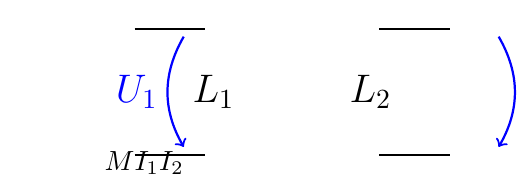
\begin{tikzpicture}[thick,scale=1, every node/.style={scale=1}]
	%\draw[help lines] (0,0) grid (4, 2);
	
	\tzTransformator{2}{1}{$M$}
	\draw (0, 1-0.8) -- (2-1.1, 1-0.8);
	\draw (0, 1+0.8) -- (2-1.1, 1+0.8);
	\draw (4, 1-0.8) -- (2+1.1, 1-0.8);
	\draw (4, 1+0.8) -- (2+1.1, 1+0.8);
	
	\node[left] at (2-0.6, 1) {\Large $L_1$};
	\node[right] at (2+0.6, 1) {\Large $L_2$};
	
	\tzCurrent{0.5}{1+0.8}{$I_1$}{r}{a}
	\tzCurrent{4-0.5}{1+0.8}{$I_2$}{l}{a}
	
	\draw [->,thick ,blue] (4, 1+0.8-0.1) to [out=-60, in=60] (4, 1-0.8+0.1); 
	\node [blue, left] at (-0.2, 1) {\Large $U_1$};
	
	\draw [->,thick ,blue] (0, 1+0.8-0.1) to [out=-120, in=120] (0, 1-0.8+0.1); 
	\node [blue, right] at (4.2, 1) {\Large $U_2$};
	
\end{tikzpicture}
